\documentclass[a4paper,10pt]{memoir}
\usepackage[italian]{babel}
\usepackage{wrapfig}
\usepackage[pdftex]{graphicx}
\usepackage{graphviz}
\usepackage{amsmath}

\usepackage{minted}

% import package
\usepackage{FrontespizioSapienza}

% declare info
\FSSTitolo{Ottimizzazione delle risorse nell'uso di servizi in background in SeismoCloud per Android}
\FSSFacolta{Facoltà di Ingegneria dell'Informazione, Informatica e Statistica}
\FSSCorso{Informatica}

\FSSCandidato{Enrico Bassetti}
\FSSMatricola{1401568}
\FSSRelatore{Emanuele Panizzi}
\FSSCorrelatore{}
\FSSAnnoAccademico{2016/2017}


% Grafico curva di scarica: cambiare nome a "Current"
% dot: grafici più grandi


\begin{document}
  
  
\frontmatter


% print title
\maketitle
\cleardoublepage

% rest of the document
\begin{abstract}
	\thispagestyle{plain}
	Sommario della tesi.
\end{abstract}
\cleardoublepage

\tableofcontents
\cleardoublepage

\mainmatter

\renewcommand\chapterheadstart{}
\renewcommand\printchaptername{}
\renewcommand\chapternamenum{}
\renewcommand\printchapternum{}
\renewcommand\afterchapternum{}
\renewcommand\printchaptertitle[1]{\chaptitlefont \thechapter. \space #1}

%\setlength{\intextsep}{1pt}%

\chapter{Il progetto SeismoCloud}

\section{I terremoti e la loro origine}


\begin{wrapfigure}{r}{0.30\textwidth}
\label{fig:litosfera}
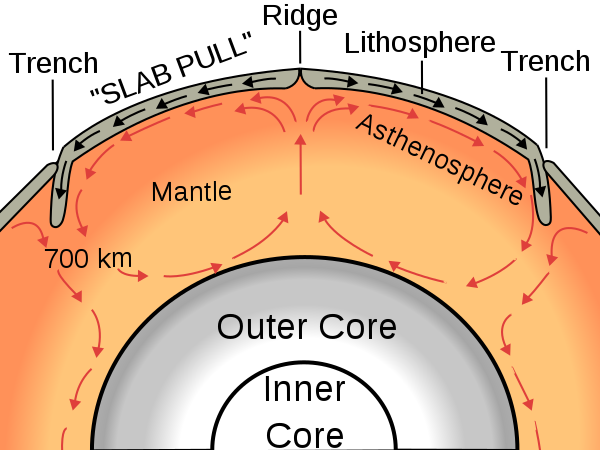
\includegraphics[width=0.30\textwidth]{introduzione/oceanic_spreading}
\end{wrapfigure}

La Terra è formata, nei primi 200 km di bordo esterno, da una zona chiamata \textit{litosfera}, di cui fa parte la \textit{crosta terrestre} con le terre emerse ed i fondali marini/oceanici. La \textit{litosfera} è divisa in parti, chiamate \textbf{placche tettoniche}, che "galleggiano" sul \textit{mantello superiore}. Queste placche sono continuamente spinte in direzioni diverse da \textit{moti convettivi} generati dalla temperatura elevata del nucleo. La zona di confine di queste placche viene chiamata \textbf{faglia}, e presenta diverse caratteristiche a seconda delle direzioni delle placche: se due placche si avvicinano, una delle due placche verrà immersa nel mantello sotto l'altra (\textit{subduzione}); se due placche si allontanano, una nuova parte della litosfera viene generata dalla roccia fusa proveniente dal mantello; infine, se due placche si muovo nella stessa direzione ma in senso opposto, siamo in presenza di \textit{margini di scorrimento}.

\begin{wrapfigure}[14]{r}{0.30\textwidth}
\caption{Mappa delle faglie italiane attive}
\label{fig:mappafaglie}
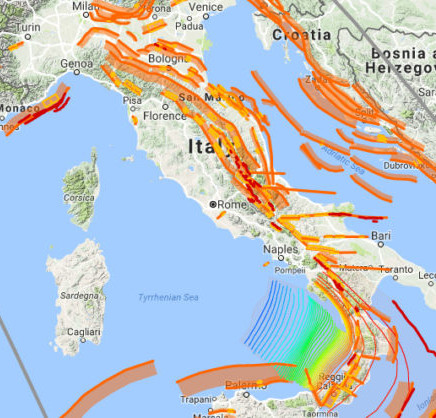
\includegraphics[width=0.30\textwidth]{introduzione/mappa_faglie_italiane2}
\end{wrapfigure}

Il movimento delle placche nei margini, tuttavia, non è libero da attrito: a seconda del materiale, della profondità e della conformazione della roccia presente nella faglia, la faglia stessa tende ad \textbf{opporsi} al movimento delle placche, accumulando energia da attrito. Quando si supera la massima forza d'attrito (per le caratteristiche ed il tipo di attrito attuato dalle due componenti rocciose), l'energia viene rilasciata repentinamente come energia meccanica (le cosiddette \textit{onde sismiche}) generando un \textit{terremoto} (o sisma).

Le onde sismiche generate da un terremoto si dividono in \textbf{Onde P} (onde di compressione, più veloci) e \textbf{Onde S} (onde trasversali, meno veloci delle onde P). Lo studio di queste due onde è importante per determinare non solo la distanza dell'ipocentro dal punto di osservazione, ma anche le caratteristiche del materiale sottostante: l'assenza di onde S è indice che tra il punto di osservazione e l'ipocentro è presente un liquido (come il magma, ad esempio), poiché le onde S non possono attraversare i liquidi\footnote{Poiché per un liquido il coefficiente di rigidità $\mu$ è nullo, la formula della velocità dell'onda S (con $\rho$ densità) $V_s = \sqrt{\mu \over \rho}$ è nulla}.

\section{Analisi e misura dei terremoti}

Per misurare l'energia sprigionata da un evento sismico, individuare il punto di origine e altre caratteristiche dell'onda, si utilizzano i \textbf{sismometri}, apparati dotati di accelerometri molto precisi, filtri e amplificatori in grado di rilevare l'accelerazione sulle tre componenti (X-Y-Z) e produrre un \textit{sismogramma} (Figura \ref{fig:sismogramma}).

\begin{figure}[p]
\caption{La rete IV - Italian Seismic Network}
\label{fig:retesensori}
\centering
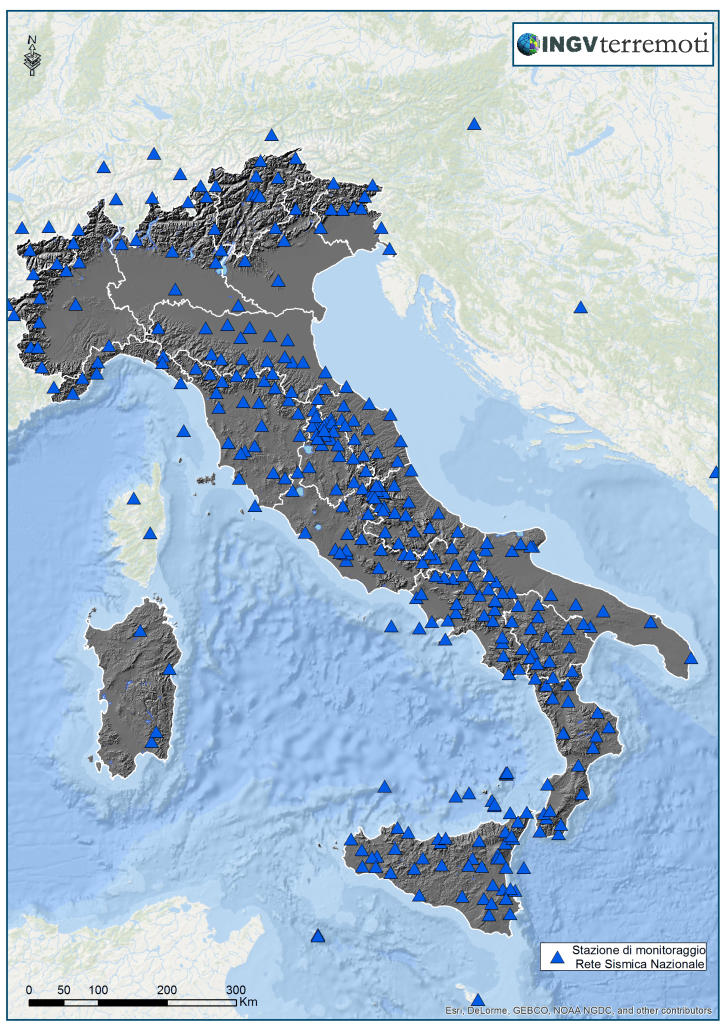
\includegraphics[width=10cm]{introduzione/rete_ingv}
\end{figure}

\begin{figure}[ht]
\caption{Esempio di sismogramma}
\label{fig:sismogramma}
\centering
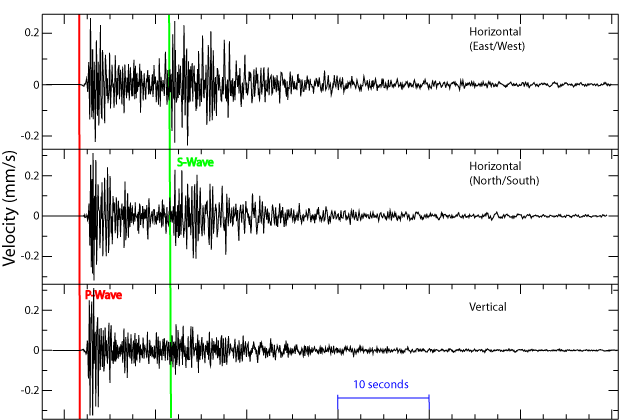
\includegraphics[width=10cm]{introduzione/seismogram}
\end{figure}

Attualmente nel mondo sono presenti diverse reti di rilevamento. Per l'Italia INGV riceve le informazioni da 27 reti sismiche (compresa la rete principale italiana \textit{IV - Italian Seismic Network}) per un totale di più di 800 sismometri (gran parte sul territorio nazionale, alcuni su paesi confinanti).

L'energia sprigionata viene misurata in \textbf{magnitudo} su una scala di valutazione chiamata \textbf{Richter}, mentre gli eventuali danni provocati vengono espressi in \textit{intensità del terremoto} tramite valori della scala \textbf{Mercalli-Cancani-Sieberg}, o MCS \footnote{Le due scale non hanno un legame diretto: un terremoto di piccola magnitudo può fare molti danni in alcune situazioni (e quindi essere di elevata intensità MCS); viceversa un terremoto di magnitudo molto elevata può avere intensità molto bassa in altre situazioni.}.

Infine possiamo distinguere il punto di origine del terremoto sotto la superficie, chiamato \textbf{epicentro}, e la proiezione di questo punto sulla superficie terrestre, chiamato \textbf{ipocentro} \footnote{Stein, Seth; Wysession, Michael (2009). An Introduction to Seismology, Earthquakes, and Earth Structure. John Wiley \& Sons. ISBN 978-1444311310}.

\begin{figure}[ht]
\caption{Epicentro, ipocentro (o focus) e faglia (\textit{fault plane})}
\label{fig:epiipo}
\centering
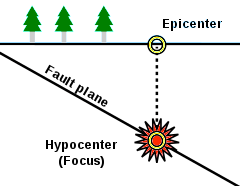
\includegraphics[scale=0.5]{introduzione/epicenter_diagram}
\end{figure}


\section{Prevedere o arginare i terremoti}

L'Italia è sottoposta, ogni giorno, ad un numero di terremoti nell'ordine del \textbf{centinaio di scosse}\footnote{Dati provenienti dal Centro Nazionale Terremoti: http://cnt.rm.ingv.it/}. Quasi tutti questi sismi sono classificati come \textit{microterremoti} (di magnitudo $<$ 2), poiché sono talmente deboli da essere percepibili solo dagli strumenti. Tuttavia, essendo l'Italia zona di confine tra la placca Europea e la placca Africana (con quest'ultima che si muove verso il Nord), la quantità di energia accumulata dalle faglie può generare terremoti in grado di infliggere ingenti danni.

Come in tutte le calamità naturali (e non), abbiamo diversi ambiti da considerare:
\begin{itemize}
\item la \textbf{prevenzione}, ovvero l'attuazione delle politiche in grado di minimizzare la probabilità che un evento accada e minimizzare il rischio all'accadere dell'evento
\item la \textbf{previsione}, ovvero l'utilizzo di tecniche e tecnologie che permettono di indicare \textit{quando un evento accadrà} (con una certa affidabilità)
\item la \textbf{gestione dell'emergenza} e del post-emergenza, ovvero delle azioni da mettere in campo durante e dopo il presentarsi di una calamità
\end{itemize}

Nella fattispecie dei terremoti, la \textbf{previsione} è tutt'ora materiale di studio da parte del mondo scientifico poiché risulta impossibile\footnote{Uyeda, Seiya; Nagao, Toshiyasu; Kamogawa, Masashi (2009-05-29), "Short-term earthquake prediction: Current status of seismo-electromagnetics", Tectonophysics, 470 (3–4): 205–213} prevedere, allo stato attuale, quando e dove accadrà il prossimo sisma\footnote{Alessandro Amato (2016). Sotto i nostri piedi. Codice edizioni, Torino. ISBN 978-8875785727}. Nel tempo, tuttavia, i vari dati raccolti riguardo ai terremoti hanno permesso di costruire delle mappe di pericolosità sismica\footnote{Pubblicate per la prima volta nel 2004 e poi aggiornate man mano: http://zonesismiche.mi.ingv.it/}, le quali indicano zone con maggiore probabilità di terremoti importanti, andando ad integrare le azioni di informazione e di formazione che fanno parte della \textbf{prevenzione}.

\begin{wrapfigure}[12]{r}{0.25\textwidth}
\centering
\label{fig:timelinecom}
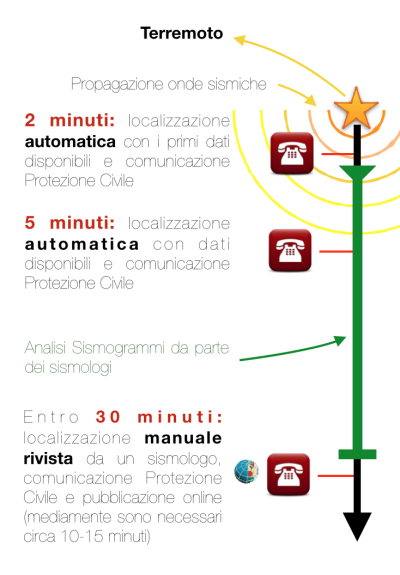
\includegraphics[width=0.25\textwidth]{introduzione/tempi_comunicazioni}
\end{wrapfigure}

Nella gestione dell'emergenza possiamo riportare quello che avviene allo stato attuale all'accadere di un terremoto, rilevato (per l'Italia) dalla rete di sismometri di INGV: nel momento in cui un sisma viene percepito da un numero congruo di stazioni di rilevamento, il sistema effettua verifiche e calcoli e, \textbf{entro due minuti}, è in grado di fornire una prima stima della magnitudo, dell'epicentro e della profondità (dati che poi vengono comunicati alla Protezione Civile). Successivamente, \textbf{entro 5 minuti} dal sisma, tutte le stazioni di rilevamento sono utilizzate per individuare le caratteristiche del terremoto in modo più preciso. Infine, \textbf{entro 30 minuti}, una verifica manuale da parte dei tecnici e ingegneri di INGV permette di avere il dato definitivo che viene di nuovo comunicato alla Protezione Civile e al pubblico\footnote{La pubblicazione avviene sul sito del Centro Nazionale Terremoti http://cnt.rm.ingv.it/ oppure tramite le pagine ufficiali sui principali Social Network}.

\section{Il progetto SeismoCloud}

Il progetto SeismoCloud nasce dalla collaborazione dall'\textbf{Università degli Studi di Roma "La Sapienza"} e l'\textbf{Istituto Nazionale di Geofisica e Vulcanologia}. L'obiettivo di questo progetto è quello di implementare un sistema di \textbf{early warning} in \textit{crowdsourcing}\footnote{Un sistema si dice in \textit{crowdsourcing} quando i dati per il suo funzionamento vengono forniti dagli stessi utenti} per i terremoti, in grado di inserirsi nel \textit{gap} presente dal momento in cui il terremoto accade, al momento in cui INGV è in grado di individuarlo. Lo scopo del sistema quindi è di individuare i terremoti \textit{in tempo reale}, alla loro apparizione nell'ipocentro, ed \textbf{anticipare} l'onda sismica (che viaggia, mediamente, ad una velocità di 5 km/s) avvertendo la popolazione nel raggio di azione del terremoto (questo sistema è chiamato, appunto, \textit{early warning}).

Già da un decennio alcuni luoghi più sensibili al terremoto si stanno dotando di infrastrutture di \textit{early detection}. Il primo Paese nel 2006 è stato il Giappone, con un sistema denominato \textbf{Earthquake Early Warning}, installato dalla \textbf{JMA} (Japan Meteorological Agency). Tale sistema è composto da 4325 sismometri su tutto il territorio giapponese\footnote{Fonte: JMA, Japan Meteorological Agency, http://www.jma.go.jp}. Il funzionamento è il seguente: quando due o più sensori individuano una scossa di terremoto, il sistema invia degli avvisi immediati attraverso radio, TV e cellulari. L'efficacia\footnote{Per "efficacia" si intende la percentuale di allarmi emessi subito dopo l'individuazione di una onda-P aventi come magnitudo $\pm1$ il valore misurato per il terremoto} di questo sistema varia dal 28\% al 76\% \footnote{Fonte: https://en.wikipedia.org/wiki/Earthquake\_Early\_Warning\_(Japan)}.

Tuttavia comporre reti di \textit{early detection} molto accurate e molto rapide, con gli stessi sismometri installati per lo studio dei terremoti, è una operazione \textbf{complessa} oltre che \textbf{costosa}: si deve posizionare il sismometro nel terreno (a volte a decine di metri di profondità), si deve mantenere un collegamento stabile e affidabile alla rete di rilevamento oltre che l'energia per far funzionare gli apparati in loco. Ecco perché SeismoCloud affronta il problema con una soluzione \textbf{crowd-sourced}: quasi tutti gli smartphone moderni sono dotati di sensori in grado di rilevare le vibrazioni (oltre che la posizione geografica) in modo relativamente accurato\footnote{Olson, Michael; Liu Annie; Faulkner Matthew; Chandy K. Mani; "Rapid Detection of Rare Geospatial Events: Earthquake Warning Applications" in DEBS '11, pp. 89-100, July 2011, ISBN 978-1-4503-0423-8}: questo permette ad ogni utilizzatore di un cellulare di essere un potenziale contributore della rete. Inoltre, con l'esplosione dell'\textit{IoT}\footnote{\textit{Internet of Things}, letteralmente \textit{internet delle cose} è l'insieme dei piccoli dispositivi, che eseguono un gruppo di funzioni ristrette (ad esempio, accendi/spegni la luce), connessi alla rete Internet} ed il costo contenuto dell'hardware di questa categoria, reti hobbystiche e comunitarie (come ad esempio le Mesh Networks) possono contribuire in modo aperto e libero.

\section{Architettura della rete SeismoCloud}

Essendo un sistema in \textit{crowdsourcing}, i dati della rete provengono dagli utenti; sono disponibili applicazioni per smartphones (Android, iOS) e per dispositivi \textit{Internet of Things} (Arduino, NodeMCU, Raspberry PI) in grado di collezionare, con apposito sensore, i dati di accelerazione nei tre assi (X, Y, e Z). La poca precisione di questi sensori (tabella \ref{table:datisensori}), in relazione ai sensori delle reti sismiche ufficiali, non permette di conoscere le componenti importanti per lo studio puntuale e storico dei fenomeni (ad esempio la distanza tra le onde P e le onde S, che richiede una analisi spettrale), tuttavia permette, con una certa affidabilità, di individuare la presenza di eventi sismici in atto se le misure singole dei vari dispositivi sono messe in relazione tra di loro.

\begin{table}[h]
\centering
\caption{Confronto tra un accelerometro della rete IV (posizionato a Latina) con un accelerometro di uno smartphone}
\label{table:datisensori}
\begin{tabular}{lll}
                    & Frequenza massima (Hz) & Sensibilità (g) \\
CMG-5T (IV.LATB) & 100 & $\pm 2.384 * 10^{-7}$ \\
ADXL345          & 50 & $\pm 3.91 * 10^{-3}$
\end{tabular}
\end{table}

Sebbene i valori siano così differenti, come si evince dalla tabella \ref{table:consumosensori}, poiché le onde sismiche hanno frequenze tra 0.1 e 15 Hz\footnote{Fonte: USGS, U.S. Geological Survey; https://earthquake.usgs.gov/learn/facts.php} la frequenza è adatta al rilevamento. La sensibilità, sebbene nettamente inferiore, è sufficiente ad individuare i terremoti in superficie\footnote{    Francesco Finazzi, Alessandro Fassò; "A statistical approach to crowdsourced smartphone-based earthquake early warning systems"; Stochastic Environmental Research and Risk Assessment.  doi:10.1007/s00477-016-1240-8}

\begin{figure}[ht]
\centering
\label{fig:scsarch}
\caption{Architettura della rete SeismoCloud}
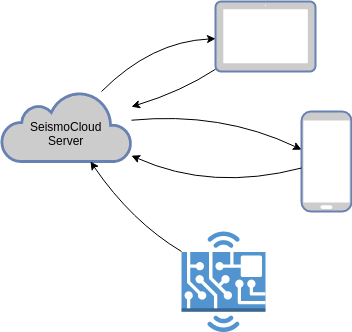
\includegraphics[width=0.5\textwidth]{introduzione/SeismoCloud_arch}
\end{figure}

Dal punto di vista utente, contribuire diventa rapido ed economico: una volta installata la \textit{app}, il sistema si avvia, acquisisce la posizione GPS ed entra a far parte della rete. Si è stimato che, per poter coprire un territorio come quello italiano occorrono dai 3000 ai 4000 sismometri, siano essi \textit{app} per cellulari o dispositivi fisici.

\section{Algoritmo di rilevamento}

\begin{wrapfigure}{r}{0.25\textwidth}
\centering
\label{fig:scsaxes}
\caption{Posizionamento assi cartesiani in uno smartphone}
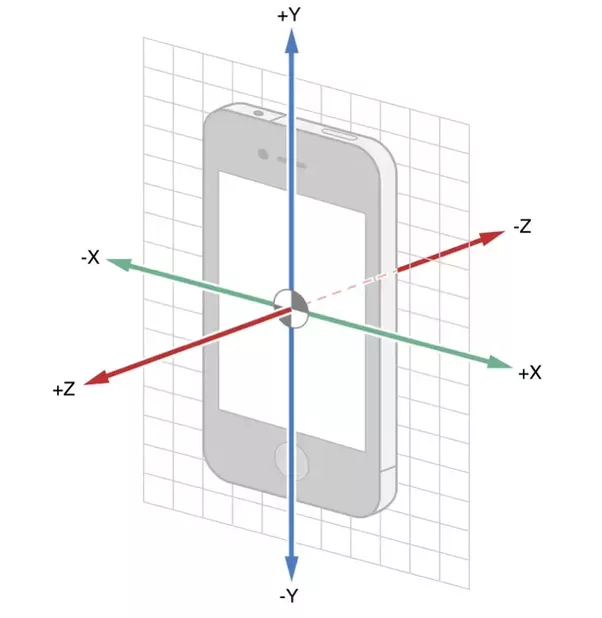
\includegraphics[width=0.25\textwidth]{introduzione/smartphone_axes}
\end{wrapfigure}

Il funzionamento del sistema è il seguente: ogni dispositivo (smartphone o dispositivo \textit{IoT}) ha almeno due stati: \textbf{ALIVE} e \textbf{QUAKE}. Un dispositivo nello stato di \textbf{ALIVE} effettua una rilevazione dell'accelerazione su ogni asse ogni $20ms$, e viene calcolata la componente del vettore risultante mediante la formula~\ref{eq:vettoreris}. Il valore viene quindi confrontato con un valore di soglia calcolato (\ref{eq:soglia}) in modo da filtrare il rumore di fondo e, se la rilevazione risulta superiore alla soglia, il dispositivo informa il server comunicando l'attuale accelerazione rilevata, la posizione geografica ed il momento della rilevazione espresso in tempo UNIX\footnote{Il "tempo UNIX" è definito come il numero di secondi dallo \textit{UNIX Epoch Time}, ovvero dal 1 Gennaio 1970} (con precisione di $\pm1ms$), e successivamene passa allo stato di \textbf{QUAKE}.

\begin{equation} \label{eq:vettoreris}
Acceleration = \sqrt{Value(X)^2 + Value(Y)^2 + Value(Z)^2}
\end{equation}

\begin{equation} \label{eq:soglia}
Threshold = Mean + Variance * \sigma
\end{equation}

Il rilevamento, con l'algoritmo sopra citato, avviene in background rispetto all'attività utente: in questo modo si consente il multitasking sul dispositivo e si mantiene l'applicazione sempre attiva in modo trasparente per l'utente.

\begin{figure}[ht]
\centering
\label{fig:scstrace}
\caption{Grafico dei dati estratti da un sensore SeismoCloud. La linea rossa rappresenta la soglia del dispositivo, le linee verdi, blu e azzurra rappresentano le eventuali soglie alternative calcolate con un valore moltiplicativo del server differente}
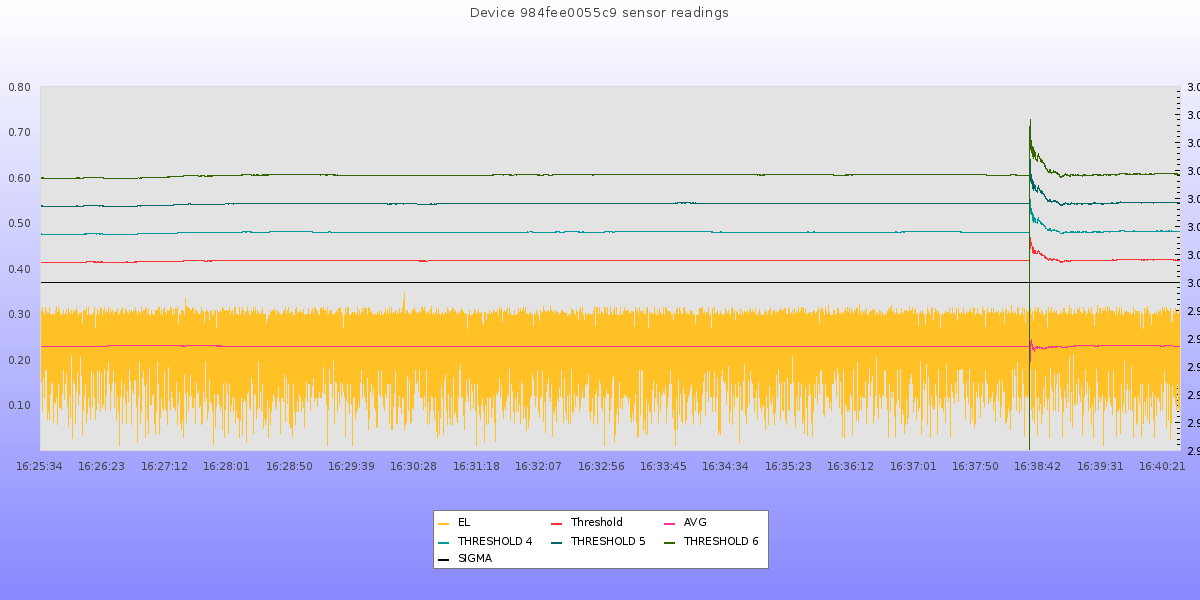
\includegraphics[width=1.5\textwidth,angle=90]{database/984fee0055c9}
\end{figure}

\chapter{Ottimizzazione energetica}

A differenza della vecchia generazione di cellulari, gli smartphones moderni fanno un uso intensivo delle risorse a bordo. In particolar modo, processori più potenti, nuove funzionalità hardware e software e multimedialità hanno reso gli smartphones moderni voraci di energia elettrica. Ecco perché è importante, quando si sviluppa codice per dispositivi \textit{mobile} (e, più in generale, per qualsiasi contesto non collegato alla griglia di distribuzione elettrica pubblica), utilizzare al meglio le capacità del dispositivo, pensando e scrivendo algoritmi \textit{battery-friendly}.

\section{I contesti di attivazione}
\label{section:contesti}

Il primo processo di ottimizzazione che è stato portato avanti riguarda i \textbf{contesti di attivazione}. Definiamo il \textbf{contesto di attivazione} come l'insieme delle variabili che rappresentano lo stato del telefono (come: stato batteria, attività utente, etc).

\paragraph{Versione base} Nella prima scrittura dell'algoritmo di rilevamento erano presenti solo due stati: \textbf{ALIVE} e \textbf{QUAKE}. All'accensione del servizio in background (avviato automaticamente dal sistema all'accensione del telefono), il telefono passava nello stato di \textbf{ALIVE} per effettuare le rilevazioni, per poi passare allo stato di \textbf{QUAKE} nel momento di una rilevazione sopra soglia. Chiaramente questo sistema prevedeva che il telefono rimanesse in orizzontale tutto il tempo. Questa prima versione è stata utilizzata in fase di test preliminare per valutare l'efficacia degli algoritmi di soglia e di rilevamento.

\begin{figure}[ht]
\centering
\label{fig:scs_sm0}
\caption{Diagramma degli stati con Alive e Quake}
\digraph[width=0.5\textwidth]{StateMachine0}{
rankdir=LR;
Quake->Alive [label="Quake motion reported"];
Alive->Quake [label="Quake motion detected"];
}
\end{figure}

\paragraph{Prima ottimizzazione} Poiché il telefono può essere in posizione non ottimale per il rilevamento, si è deciso di procedere all'attivazione del servizio solo quando il telefono si trova in \textbf{posizione orizzontale} (con le tecniche specificate nella sezione \ref{section:sensori}). Questa modifica permette di risparmiare le risorse, ed in particolar modo la batteria (tramite la diminuzione della pressione sulla CPU e memoria), quando il telefono è usato dall'utente oppure non poggiato su una superficie piana (ad esempio, il telefono si trova in una tasca oppure in una borsa). Per stabilire le soglie dei valori da considerare come "rotazione" si è stabilito un \textit{range} di rotazione assoluto rispetto al piano orizzontale, ed un offset di rotazione relativo. \textbf{Questo ci permette di individuare sia il posizionamento non favorevole del telefono, sia una sua rotazione o spostamento in modo repentino}. Quest'ultimo caso è importante perché ci ha permesso di ridurre al minimo i falsi positivi relativi all'azione dell'utente (ad esempio il prendere in mano il telefono) su un cellulare posizionato, fino a quel momento, in orizzontale. Abbiamo quindi introdotto un nuovo stato, lo stato di \textbf{MOVE}. La transizione da uno stato all'altro è determinata dai controlli fatti sui valori dei sensori.

\begin{listing}[H]
\caption{Codice di gestione della rotazione (alcune linee sono state accorpate per la stampa)}
\begin{minted}[mathescape,
               linenos,
               numbersep=5pt,
               gobble=0,
               frame=lines,
               framesep=2mm]{java}
boolean inRotation = Math.abs(gravity[2]) < gravityThreshold
		|| !(gravity[0] > -1 && gravity[0] < 1)
		|| !(gravity[1] > -1 && gravity[1] < 1);
if (isMoving)
	// Siamo in movimento - MOVE - valuto una transizione MOVE->FLAT
	if (accelerometerIntensity < 0.3 && !inRotation) {
		// I valori sono buoni per considerare la posizione come FLAT
		if (++countFlat > 5) {
			// Soglia di 5 valori OK per FLAT, passaggio a FLAT
			switchToMove(false); countFlat = movingLastMs = 0;
			seismometer.reset();
			// Informo il server che sono di nuovo OK
			WebApiInterface.alive(...);
		}
	} else countFlat = 0; // riparto da zero per MOVE->FLAT
else // Siamo in posizione stabile - FLAT - controllo se siamo in rotazione
	if (inRotation) {
		// Valori fuori scala per FLAT - transizione FLAT->MOVE
		goToMoving(); isQuake = 0;
		movingLastMs = System.currentTimeMillis();
	} else if (seismometer.tick(accelerometerIntensity)
			&& magneticValues[0] != 0 && magneticValues[1] != 0
			&& magneticValues[2] != 0) {
		// Calcolo la rotazione
		float[] rot = computeOrientation(); oldRotation = rotation;
		rotation = 1000*sqrt(rot[0]*rot[0]+rot[1]*rot[1]+rot[2]*rot[2]);
		deltaRot = (oldRotation==0.0d)?0.0d:abs(rotation-oldRotation);
		countFlat = 0;
		if (deltaRot > 75.0) {
			// il telefono e' in rotazione, quindi si va in MOVE
			goToMoving(); movingLastMs = System.currentTimeMillis();
		} else if (!inQuakeCondition) {
			// Niente rotazione pero' valore sopra soglia
			seismometer.addValueToAvgVar(accelerometerIntensity);
			Double d = Math.floor(System.currentTimeMillis()/1000D);
			WebApiInterface.terremoto(d.intValue(), location);
			magneticValues = new float[]{0, 0, 0};
			oldRotation = rotation = deltaRot = 0.0d;
			isQuake = System.currentTimeMillis();
			stopCause = StopCause.QUAKE;
		}
	} else {
		countFlat++;
		// Aggiorno la soglia
		if (!inQuakeCondition)
			seismometer.addValueToAvgVar(accelerometerIntensity);
		// Keep alive
		if (System.currentTimeMillis() - timerAlive > 15 * 60 * 1000) {
			WebApiInterface.alive(...);
			timerAlive = System.currentTimeMillis();
		}
	}
\end{minted}
\end{listing}

\begin{figure}[ht]
\centering
\label{fig:scs_sm1}
\caption{Diagramma degli stati con Alive, Quake e Move}
\digraph[width=0.7\textwidth]{StateMachine1}{
Start [style=invis];
rankdir=LR;
Start->Alive [label="Service started"];
Quake->Alive [label="Quake motion reported"];
Alive->Quake [label="Quake motion detected"];
Alive->Move  [label="Rotation off-range"];
Move->Alive  [label="Rotation normal"];
}
\end{figure}

\paragraph{Seconda ottimizzazione} Una seconda ottimizzazione è stata apportata dallo spegnimento del servizio per un periodo stabilito quando il telefono si trova in uno stato non utile (\textit{MOVE} ad esempio). E' stato introdotto lo stato di \textbf{MOVE\_BACKOFF}, dove il servizio viene portato dopo un periodo di permanenza in \textit{MOVE}. Questo stato prevede lo \textbf{spegnimento} del servizio, con il rilascio di tutti i WakeLocks\footnote{Un "WakeLock" è un meccanismo di segnalazione, al sistema operativo Android, che permette di richiedere di lasciare attivi alcuni sottosistemi, come lo schermo od il chip WiFi - se nessuno richiede un WakeLock infatti, il cellulare va in uno stato di quiete per cui la CPU principale, il WiFi e altri chip vengono spenti}. Per decidere quando riattivare il servizio (e controllare se ci sono le condizioni per passare allo stato di \textit{ALIVE}) viene utilizzato un algoritmo di \textbf{backoff esponenziale}: al primo passaggio allo stato di \textit{MOVE\_BACKOFF} il tempo per il risveglio (e quindi il prossimo controllo) viene impostato a 30 secondi. Successivamente, se il controllo per il passaggio da \textit{MOVE} as \textit{ALIVE} fallisce (quindi rimaniamo dentro \textit{MOVE}) il tempo di \textit{MOVE\_BACKOFF} viene raddoppiato ogni volta, fino ad un massimo di 900 secondi.

In questo modo il servizio, durante il periodo di \textbf{MOVE\_BACKOFF}, non consuma risorse e non detiene nessun tipo di WakeLock, permettendo quindi al telefono di andare in \textit{stand-by} e gestire il sistema come se SeismoCloud non fosse installato. \textbf{Il consumo determinato dalla nostra app mentre il telefono è in uso, oppure in posizione non orizzontale, è zero}. Il risveglio invece è gestito dal sistema operativo \textbf{Android}, il quale gestisce in modo ottimizzato gli interrupt basati sul tempo (come questo per la riattivazione del servizio), spesso (sui telefoni che lo supportano) con un chip dedicato a consumo molto ridotto.

\begin{figure}[ht]
\centering
\label{fig:scs_sm2}
\caption{Diagramma degli stati con Alive, Quake, Move e Move\_Backoff}
\digraph[width=\textwidth]{StateMachine2}{
rankdir=LR;
Start [style=invis];
Start->Alive [label="Service started"];
Quake->Alive [label="Quake motion reported"];
Alive->Quake [label="Quake motion detected"];
Alive->Move  [label="Rotation off-range"];
Move->Alive  [label="Rotation normal"];
Move_Backoff->Move  [label="Interrupt (timeout)"];
Move->Move_Backoff  [label="Persistent Move state"];
}
\end{figure}

\paragraph{Controllo della localizzazione} Una ulteriore ottimizzazione è stata l'introduzione del controllo sulla effettiva disponibilità del segnale GPS o dalla localizzazione da rete (utilizzata qualora non sia presente il GPS sul dispositivo, oppure non sia abilitato o ancora non sia presente il segnale satellitare): sia in fase iniziale, sia durante il funzionamento (stato \textbf{ALIVE}), il sistema controlla l'effettiva presenza di una localizzazione valida (sia essa il GPS o una posizione acquisita tramite rete cellulare). Questo permette di individuare diverse situazioni a noi sfavorevoli:

\begin{itemize}
\item \textbf{Disattivazione del sensore di localizzazione} da parte dell'utente (tramite apposita opzione di Android) oppure perdita del segnale
\item \textbf{Spostamento} del telefono (inteso come identificazione dello spostamento geografico dell'utente, ad esempio quando si muove in auto)
\end{itemize}

In entrambi i casi il servizio non è più in grado di fare affidamento alla posizione memorizzata, dunque entra nello stato di \textbf{MOVE\_BACKOFF}, dove continuerà ad essere fino alla riaccensione del sensore di localizzazione (nel primo caso) o ad una posizione valida e fissa (nel secondo caso). Questo ha permesso di ridurre, come da test effettuati, il consumo di batteria in particolari condizioni: ad esempio posizionare il telefono sul cruscotto di una automobile, o su di un tavolino del treno, avrebbe comportato l'attivazione del servizio a causa della posizione orizzontale, tuttavia i dati di accelerazione sarebbero stati ovviamente inutili ai fini dell'indentificazione del terremoto. Dunque, \textbf{con questa nuova aggiunta il sistema è in grado di rilevare questi casi} e si pone nello stato corretto.

Poiché la precisione della localizzazione via rete cellulare è molto variabile (dai pochi metri a decine di km), è stato stabilito di non considerare localizzazioni via rete cellulare che hanno un errore maggiore di $\pm250$ metri.

\paragraph{Controllo della connessione dati} Un altro fattore importante per una buona rilevazione è la presenza della connessione di rete (Wi-Fi o rete cellulare). Qualora venga a mancare la connessione Internet non si potrà avvertire per tempo il server: il sistema è quindi portato nella posizione di \textbf{MOVE\_BACKOFF} con l'algoritmo sopra citato. Questo permette di risparmiare batteria quando il segnale è assente.

\paragraph{La batteria} Infine, è stata fatta una analisi sulla batteria e sul consumo. In prima istanza è stato considerato lo status di "\textbf{risparmio energia}" che Android attiva nel momento in cui la batteria raggiunge un valore prefissato (in genere, a meno di cambiamenti fatti dall'utente, il valore è il 15\% della capacità). Grazie ad un \textit{handler} viene intercettato questo evento e viene posto il servizio nella fase di \textbf{MOVE\_BACKOFF} indipendentemente dalle condizioni favorevoli sopra citate. Dopodiché si è provveduto ad effettuare uno studio approfondito, con diversi test, meglio specificata nel capitolo \ref{section:batteria}.

\paragraph{Conclusioni} Abbiamo quindi definito una serie di variabili che compongono il nostro \textbf{contesto di attivazione}, ovvero:

\begin{itemize}
\item Rotazione/posizione favorevole o no alla lettura del dato
\item Persistenza della posizione sfavorevole nel tempo
\item Presenza o meno della localizzazione GPS
\item Presenza o meno di uno spostamento geografico
\item Presenza o meno della rete Internet
\item Status di risparmio energetico del sistema operativo (capacità batteria rimanente)
\end{itemize}

Questa definizione ci permette di stabilire, come abbiamo fatto, una istanza del contesto per la quale è favorevole attivare il servizio (localizzazione presente, posizione orizzontale, etc.), permettendo così un risparmio notevole (come evidenziato dalla tabella \ref{table:tempoutilizzo} e dalla figura \ref{fig:usagechart}). Nella figura \ref{fig:scs_sm3} invece è rappresentato il diagramma degli stati dopo le ottimizzazioni esposte. L'impatto di queste e successive ottimizzazioni sulla batteria è possibile vederlo nella figura \ref{fig:batterychart} a pagina \pageref{fig:batterychart}.

\begin{table}[h]
\centering
\caption{Tempo di utilizzo delle risorse (media giornaliera)}
\label{table:tempoutilizzo}
\begin{tabular}{lllll}
& \textbf{Servizio attivo} & \textbf{Servizio inattivo} & \textbf{Telefono spento} &  \\
Algoritmo originale   & 18 ore e 24 min  & mai              & 5 ore 36 min &  \\
Algoritmo ottimizzato & 6 ore e 36 min   & 11 ore e 48 min  & 5 ore 36 min &
\end{tabular}
\end{table}

\begin{figure}[ht]
\centering
\caption{Diagramma degli stati per i contesti di attivazione}
\label{fig:scs_sm3}
\digraph[width=\textwidth]{StateMachine3}{
rankdir=LR;
Start [style=invis];
Start->Alive [label="Service started"];
Quake->Alive [label="Quake motion reported"];
Alive->Quake [label="Quake motion detected"];
Alive->Move  [label="Rotation off-range"];
Move->Alive  [label="Rotation normal"];
Move_Backoff->Move  [label="Interrupt (timeout)"];
Move->Move_Backoff  [label="Persistent Move state"];
Alive->Move_Backoff  [label="Location unavailable/move"];
Alive->Move_Backoff  [label="Android Power safe mode"];
Alive->Move_Backoff  [label="Internet unavailable"];
}
\end{figure}

\begin{figure}[ht]
\centering
\caption{Comparazione (valori medi in un giorno) dell'utilizzo delle risorse CPU e sensori da parte degli algoritmi con (\textit{Current}) e senza (\textit{Original}) contesto di attivazione: si può notare come il tempo di inattività in blu (\textbf{MOVE\_BACKOFF}) sia una porzione notevole del tempo totale}
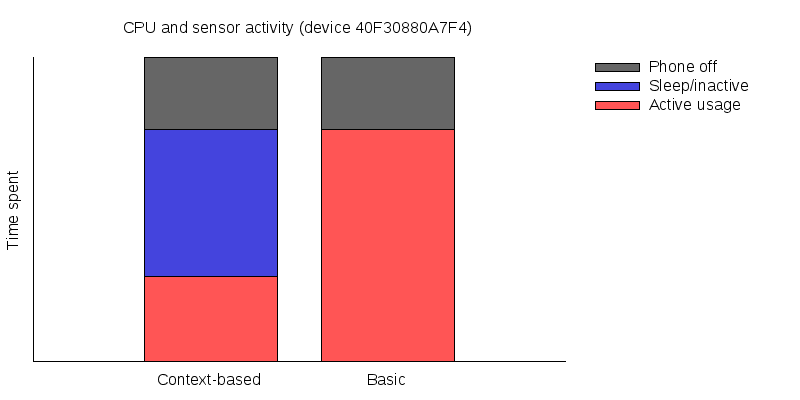
\includegraphics[width=\textwidth]{database/usageplot}
\label{fig:usagechart}
\end{figure}


\section{La comunicazione con il front-end}

Qui si descrive la politica utilizzata per mantere l'applicazione attiva (notifica permanente) poiché Android pone le applicazioni in sleep. Si spiega anche il wakelock sulla CPU, la sospensione dell'aggiornamento dati in background delle activity quando non sono in vista.

\section{I sensori}
\label{section:sensori}

Ogni modello di smartphone Android è dotato di un numero variabile di sensori, a seconda del produttore e della fascia di prezzo in cui si vuole inserire il dispositivo. Mentre i modelli \textit{top} di gamma hanno un numero impressionante di sensori (ad esempio il Samsung S4 è dotato di ben 34 sensori - virtuali e non - accessibili all'utente), altri telefoni hanno solo alcune tipologie di sensori.

\paragraph{Di cosa abbiamo bisogno} Il servizio della App SeismoCloud deve individuare le vibrazioni, quindi sicuramente è necessario l'\textbf{accelerometro}. Inoltre deve individuare, come abbiamo visto nel capitolo precedente, quando si trova poggiato con una inclinazione non utile per la rilevazione: per questo abbiamo bisogno del \textbf{giroscopio}. Inizialmente il codice fu scritto per questi due sensori, ma effettuando i test della applicazione abbiamo scoperto che molti telefoni di fascia "economica" sono sprovvisti del giroscopio. Poiché questi modelli di telefono sono i più diffusi, è stato effettuato uno studio per capire come poter ovviare al problema.

\paragraph{La fascia economica} Il problema della mancanza del giroscopio probabilmente è molto conosciuto agli sviluppatori Android, i quali hanno messo a disposizione una libreria che sfrutta un altro sensore, diffuso tanto quanto l'accelerometro: il \textbf{magnetometro}. Grazie ai valori letti dal magnetometro e dall'accelerometro, è possibile calcolare l'attuale rotazione del telefono (rispetto al piano orizzontale).

\begin{listing}[H]
\caption{Porzione di codice che calcola la rotazione in base ai dati del magnetometro e dell'accelerometro}
\begin{minted}[mathescape,
               linenos,
               numbersep=5pt,
               gobble=0,
               frame=lines,
               framesep=2mm]{java}
private synchronized float[] computeOrientation() {
   float[] rotationMatrix = new float[16];
   float[] iMatrix = new float[16];
   float[] orientation = new float[3];
   // "gravity" contiene i valori dell'accelerometro
   // "magneticValues" contiene i valori del magnetometro
   if (SensorManager.getRotationMatrix(rotationMatrix, iMatrix,
                                       gravity, magneticValues)) {
      SensorManager.getOrientation(rotationMatrix, orientation);
   }
   return orientation;
}
\end{minted}
\end{listing}

\paragraph{Il calcolo della rotazione tramite magnetometro} [indicare qui come avviene dentro le API fornite da Android]

\paragraph{Alla ricerca dell'ottimizzazione} Poiché il magnetometro e l'accelerometro forniscono un dato affidabile quanto basta per rilevare la rotazione sul piano orizzontale del telefono, e poiché la frequenza di rilevazione del magnetometro è impostabile (al contrario del giroscopio), si è deciso di procedere con un tentativo di ottimizzazione che includesse due fasi nella fase \textbf{ALIVE} (fase di rilevamento dei valori dell'accelerometro): sono state introdotte le fasi \textbf{ALIVE\_SLOW} e \textbf{ALIVE\_FAST}. Ogni fase registrava sensori differenti con frequenze differenti:

\begin{itemize}
\item \textbf{ALIVE\_SLOW}: registrati \textbf{magnetometro} e \textbf{accelerometro} con tempi di rilevazione di $100ms$
\item \textbf{ALIVE\_FAST}: registrati \textbf{giroscopio}, se presente, altrimenti \textbf{magnetometro}, e \textbf{accelerometro} con tempi di rilevazione di $50ms$
\end{itemize}

Inizialmente veniva attivata la fase \textbf{ALIVE\_SLOW}. Successivamente, ad una attività del magnetometro sopra soglia, il servizio passava allo stato di \textbf{ALIVE\_FAST} e controllava il dato del giroscopio (se presente, altrimenti di nuovo del magnetometro).

\begin{figure}[ht]
\centering
\caption{Diagramma degli stati per \textbf{ALIVE\_FAST} e \textbf{ALIVE\_SLOW}}
\label{fig:scs_sm4}
\digraph[width=0.7\textwidth]{StateMachine4}{
rankdir=LR;
Start [style=invis];
Start->Alive_Slow [label="Service started"];
Alive_Fast->Alive_Slow [label="No significant rotation detected"];
Alive_Slow->Alive_Fast  [label="Significant rotation detected"];
}
\end{figure}

L'ipotesi era che questa diminuzione di frequenza fosse apprezzabile, sia dal punto di vista del carico sulla CPU, sia dal punto di vista del carico della batteria.

\paragraph{Test finali e conclusioni} Tuttavia, successivi test hanno rivelato come questa differenza ipotizzata tra le due frequenze di lettura sia praticamente nulla. Inoltre, la mancanza del giroscopio in alcuni telefoni aveva significato scrivere più codice per gestire tutti i casi. Infine, una indagine più approfondita dal punto di vista energetico ha svelato\footnote{http://www.edn.com/design/sensors/4431747/Lower-power-and-cost-for-Android-device-motion-sensing-using-mCube-s-iGyro-} \footnote{https://www.sparkfun.com/pages/accel\_gyro\_guide} che \textbf{il giroscopio ha un consumo enormemente maggiore rispetto all'accelerometro e al magnetometro}, i quali tra l'altro risultano spesso integrati in un solo chip (tabella \ref{table:consumosensori}). Si è quindi deciso di procedere eliminando il requisito del giroscopio e di mantenere solo una fase di \textbf{ALIVE} contenente la registrazione dei sensori \textbf{accelerometro} e \textbf{magnetometro} alla velocità stabilita.

\begin{table}[h]
\centering
\caption{Comparazione sul consumo delle tipologie di sensori più comuni per le due tipologie}
\label{table:consumosensori}
\begin{tabular}{lllll}
& \textbf{In fase di misura} & \textbf{Stand-by} & \\
Accelerometro + Magnetometro \\
ADXL345\footnote{integrati} & $40 \mu A$ & $0.1 \mu A$ &  \\
Giroscopio \\
L3G4200D\footnote{https://cdn.sparkfun.com/datasheets/Sensors/Gyros/3-Axis/CD00265057.pdf} & $6.1mA$ & $0.2mA$ &
\end{tabular}
\end{table}

\section{La curva di scarica}
\label{section:batteria}

Una risorsa molto importante, dal punto di vista degli utenti, è la batteria: mentre i vecchi telefoni avevano una autonomia di giorni se non settimane, i nuovi smartphones spesso richiedono una o più ricariche al giorno. L'obiettivo quindi è quello di portare il servizio di rilevamento dell'applicazione SeismoCloud ad impattare il meno possibile sul consumo totale, anche sacrificando periodi di rilevazione. Il motivo di questa scelta è semplice: un impatto ridotto dal punto di vista energetico può portare l'applicazione ad essere installata su più dispositivi, compensando il tempo di attività che verrebbe a mancare con l'introduzione dell'algoritmo esposto in questa sezione.

\paragraph{La curva di scarica} In parte, le ottimizzazioni già presentate nella sezione \ref{section:contesti} hanno portato ad un risparmio energetico; tuttavia si è voluto studiare un sistema più "\textit{aggressivo}" per portare i consumi al minimo possibile. Sono partito quindi da quello che è il principale requisito per l'utente: \textbf{il telefono deve arrivare a fine giornata}, ovvero nessuna applicazione deve consumare così tanto da rendere il telefono scarico prima di avere una fonte di energia.

Poichè in quasi tutti i casi le persone si trovano in un luogo con corrente elettrica per cena, facendo una rapida analisi sui dati presenti sul \textit{database} è stato identificato, come \textit{target}, una \textbf{carica residua del 15\% alle ore 20:00}, partendo dal 100\% alle ore 08:00. E' stata quindi calcolata una curva lineare di scarica, con lo scopo di tenere il servizio attivo solo quando è sopra la soglia.

\begin{equation}
\gamma = {85 \over 720}
\end{equation}

\begin{equation}
\lambda = \text{hour} * 60 + \text{minutes}
\end{equation}

\begin{equation}
	\\
    Threshold =
    \begin{cases}
        100 & \text{if hour} < 8\\
        {100 - ((\lambda - 480) * \gamma)} & \text{otherwise.}
    \end{cases}
\end{equation}

Dove:
\begin{itemize}
\item $\gamma \in Z^+$ rappresenta il \textit{rate} di perdita della capacità della batteria per minuto nella fascia 8-20
\item $\lambda \in N^+$ rappresenta il numero di minuti a partire dalla mezzanotte del giorno
\item $Threshold \in Z^+$, $0 <= Threshold <= 100$ è il valore attuale di capacità della batteria (espresso in percentuale) previsto per l'orario attuale
\end{itemize}

\begin{figure}[ht]
\centering
\caption{Comportamento atteso: la carica del cellulare (verde, in questo caso simulata) non deve mai scendere sotto la curva di scarica calcolata (rosso)}
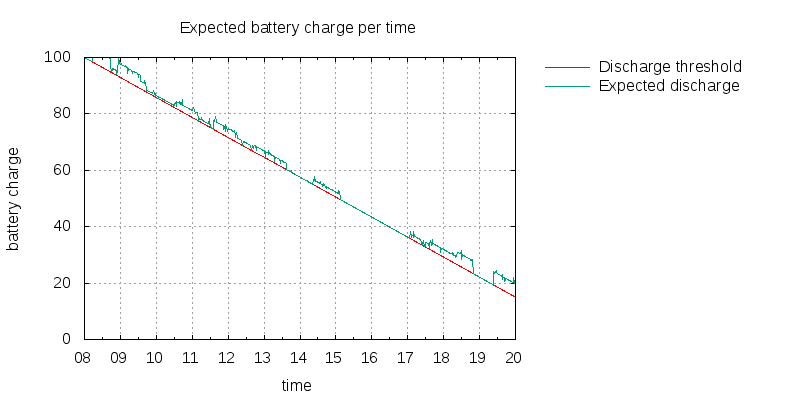
\includegraphics[width=\textwidth]{database/expectedplot}
\label{fig:expectedchart}
\end{figure}

Dopo averla applicata sui dispositivi di test, abbiamo subito notato un enorme cambiamento: nonostante un tempo di attività leggermente inferiore a causa dei distacchi per rispettare la soglia (cosa che, ovviamente, varia da telefono a telefono a seconda della capacità della batteria, delle applicazioni installate, dell'hardware del telefono e dell'utilizzo), il consumo evidenziato dai dati sul \textit{database} è nettamente migliore, come mostrato nella figura \ref{fig:batterychart}.

\begin{figure}[h]
\centering
\caption{Capacità residua batteria (media) prima e dopo l'ottimizzazione: \textit{Basic} rappresenta l'algoritmo di base senza ottimizzazioni, \textit{Context-based} rappresenta l'algoritmo che utilizza solo i contesti di attivazione, mentre \textit{Current} rappresenta l'algoritmo corrente, che sfrutta sia i contesti di attivazione che la curva di scarica}
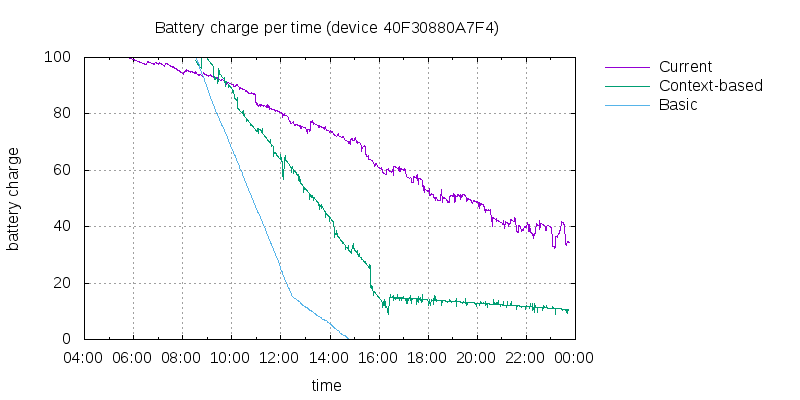
\includegraphics[width=\textwidth]{database/batteryplot}
\label{fig:batterychart}
\end{figure}


\begin{listing}[H]
\caption{Porzione di codice che calcola la curva di scarica e indica se procedere o no con il servizio}
\begin{minted}[mathescape,
               linenos,
               numbersep=5pt,
               gobble=0,
               frame=lines,
               framesep=2mm]{java}
// Orario di inizio
private static final Double T0 = 8 * 60.0;
// Orario di fine
private static final Double T1 = 20 * 60.0;
// Carica iniziale
private static final Integer B0 = 100;
// Ratio di scarica
private static final Double R0 = (100.0 - 15.0) / (T1 - T0);
/**
 * Calcola il valore atteso della batteria all'orario corrente
 */
public static Double expectedBattery() {
	Calendar c = Calendar.getInstance();
	if (c.get(Calendar.HOUR_OF_DAY) < 8) {
		return 100.0;
	}
	Integer Tx = c.get(Calendar.HOUR_OF_DAY) * 60 + c.get(Calendar.MINUTE);
	return Math.floor(B0 - ((Tx - T0) * R0));
}
/**
 * Controlla se ci sono le condizioni per proseguire
 * (caricabatterie collegato oppure valore batteria sopra curva)
 */
public static boolean shouldProceedWithService(Context ctx) {
	if (BatteryLevelReceiver.isPowerSupplyConnected(ctx)) {
		return true;
	}
	Float now = Utils.getBatteryLevel(ctx);
	return now == 0 || (expectedBattery() <= now && now > 15.0);
}
\end{minted}
\end{listing}

\chapter{Ottimizzazione della rete}

\section{MQTT}

Si spiega come l'introduzione dell'MQTT abbia ridotto il carico sulla rete per lo scambio dati con il server.

\section{Pushback}

Parlare del meccanismo di Pushback per l'invio dei dati (ad esempio survey) in background in modo ottimizzato in caso di problemi di rete (invio asincrono).

\chapter{Ottimizzazione dell'uso di memoria nel codice}

Per ogni valore rilevato nello stato \textit{ALIVE}, inoltre, vengono aggiornati i seguenti valori:
\begin{equation}
\Delta = Acceleration - \rho
\end{equation}
\begin{equation}
\rho = \rho + {\Delta \over |detections|}
\end{equation}
\begin{equation}
\sigma = \sigma + \Delta * (Acceleration - \rho)
\end{equation}
\begin{equation}
Threshold = \rho + (\sqrt{\sigma \over (|detections|-1)} * \alpha)
\end{equation}

dove: \begin{itemize}
\item $Acceleration \in Z^+$ rappresenta il valore di accelerazione attuale
\item $\rho \in Z^+$ è la media dei valori delle rilevazioni, e $\sigma \in Z^+$ lo scarto quadratico medio, entrambi calcolati mediante un \textit{algoritmo online}\footnote{Un algoritmo viene definito \textit{online} se è in grado di processare un oggetto di input per volta (mantenendo l'invariante che il risultato rappresenta il valore atteso), potenzialmente per un numero infinito di oggetti}
\item $Threshold \in Z^+$ rappresenta la soglia di confronto per il valore di accelerazione, utilizzata per decidere se è da informare il server
\item $\alpha \in Z^+$ rappresenta un valore moltiplicativo fornito dal server (aggiornato a seguito, ad esempio, di eccessive segnalazioni o soglia troppo alta)
\end{itemize}

Qui si descrive la politica utilizzata, nella costruzione del codice, per minimizzare lo spreco di memoria (esempio: media/varianza mobile).

\clearpage

\begin{figure}[ht]
\centering
\caption{Diagramma di flusso del servizio SeismoCloud}
\label{fig:serviceflowdiagram}
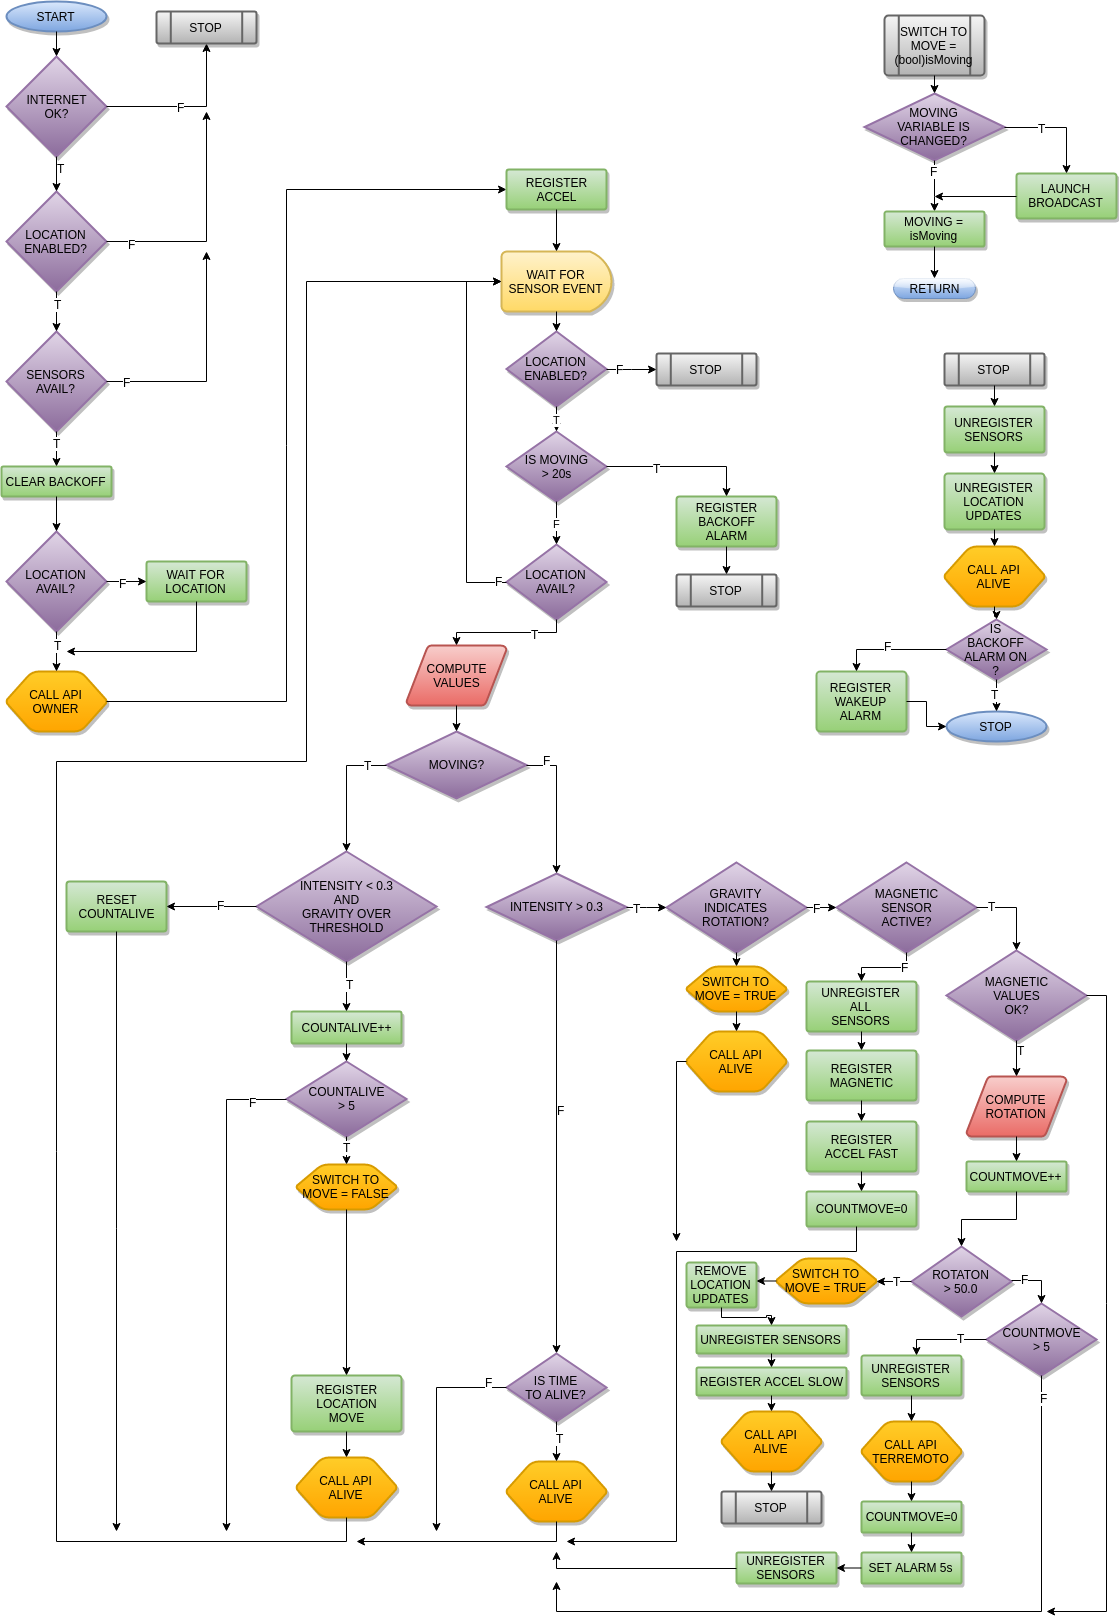
\includegraphics[width=\textwidth]{SeismoCloud_flowdiag}
\end{figure}

%
%\chapter{Sviluppo e test}
%
%Si spiega l'adozione di particolari meccanismi per la gestione ottimizzata del processo di sviluppo:
%
%\begin{itemize}
%\item Utilizzo della libreria ACRA per l'immediata segnalazione di errori della app (da produzione)
%\item Utilizzo della libreria LeakCanary per la ricerca di memory leak
%\item Utilizzo delle librerie Parceler e Android Annotations per ridurre la quantità di codice ridondante
%\item Sistemi di controllo versione: branch per funzionalità, sviluppo parallelo
%\item Continuos integration per la verifica dei build ed instrumentation test
%\item Verifica del codice tramite SonarQube per aderenza agli standard Java/Android e risultati di analisi statica del codice
%\end{itemize}

\chapter{Conclusioni e sviluppi futuri}

\begin{itemize}
\item Utilizzo di un sistema di spegnimento controllato dal server per l'ottimizzazione geografica
\item Utilizzo di sensori dedicati (es. Samsung Significant Motion Sensor) per il wake-up
\item Riscrittura parti critiche in codice nativo per l'esecuzione ottimizzata e rapida (con conseguente aumento del periodo di idle del telefono)
\item Implementazione delle tecniche descritte in \textit{"Energy-Accuracy Trade-off for Continuous Mobile Device Location"; Kaisen Lin, Aman Kansal, Dimitrios Lymberopoulos, Feng Zhao; MobiSys '10 Proceedings of the 8th international conference on Mobile systems, applications, and services; ISBN: 978-1-60558-985-5}
\end{itemize}

\end{document}
